\documentclass{article}
\usepackage{graphicx}
\usepackage{amsmath}
\usepackage{amssymb}
\usepackage{geometry}
\usepackage{tikz}


\geometry{a4paper, margin=1in}

\title{CS 440 Assignment 1 - Questions 2 \& 5}
\author{Saul Santiago Rodriguez}
\date{\today}

\begin{document}

\maketitle

\section*{Question 2: The Effect of Breaking Ties using G-Values}

\subsection*{Methodology}
We implemented one version of the Repeated Forward A* algorithm with a variable that determined the cell prioritization:
\begin{itemize}
    \item \textbf{A* search (a\_star\_search)}: The agent plans a path from its current position to the goal. The heuristic used is the Manhattan distance from a node $n$ to the goal.  
    \item \textbf{Sign (variable)}: Int that is either -1 or +1. Used to determine if expansion should prioritize cells with a large g value (-1 is used) or with a small g value (+1 is used). 
\end{itemize}
In both prioritization cases, ties in f-values were broken by implementing a constant variable $c$, a whole number that is bigger than any possible g-value.

\[ c = l(m) + w(m) + 1 \]

\begin{center}
Where $l(m)$ is the $length$ of the maze, $w(m)$ is the $width$, and +1 makes the constant larger than any possible g-value.
\end{center} 

\subsection*{Results}
Experiments were ran on 50 randomly generated gridworlds of size 101x101. The table below summarizes the average performance of each prioritization method by comparing the number of cells expanded and runtime.

\begin{center}
\begin{tabular}{|l|r|r|r|r|r|}
\hline
\textbf{Maze} & \textbf{Solvable} & \textbf{Large G Cells Exp.} & \textbf{Small G Cells Exp.} & \textbf{Large Replans} & \textbf{Small Replans} \\
\hline
Maze 0  & False & 22906  & 338397 & 142 & 152 \\
Maze 1  & False & 17763 & 262180 & 79  & 80  \\
Maze 2  & False & 17085 & 185962 & 83  & 83  \\
Maze 3  & True  & 13190 & 256344 & 135 & 135 \\
Maze 4  & True  & 9605   & 320602 & 96  & 101 \\
... & ... & ... & ... & ... & ... \\
Maze 49 & False & 1     & 1      & 0   & 0   \\
\hline
\textbf{Average} & \textbf{ --- } & \textbf{8637.8} & \textbf{158401.0} & \textbf{62.8} & \textbf{63} \\
\hline
\end{tabular}
\end{center}

\subsection*{Analysis}
\textbf{Observation:} Prioritizing expansion based on the cell with the Largest G values consistently proved to expand about 95\% less cells than prioritizing cells with Small G values (which on average expanded almost 18 times more cells than Large G prioritization). To reduce the impact of variance in cell exploration due to differences in implementations, a singular helper function was developed that would perform the same maze exploration but change prioritization based on a variable passed. \\

\noindent While there is a substantial difference in the cells expanded, the re-plan counts between both prioritization methods average out to be almost the same number of 63. In both tie-breaking methods, the agent often runs into the same walls due to pathing, thus producing nearly identical plans. There are also mazes that only expand 1 cell before being deemed unsolvable. This is due to the right (0,1) and bottom cell (1,0) both landing the 0.30\% odds of being blocked cells. These mazes were still included in the calculations.

\noindent \begin{center}
    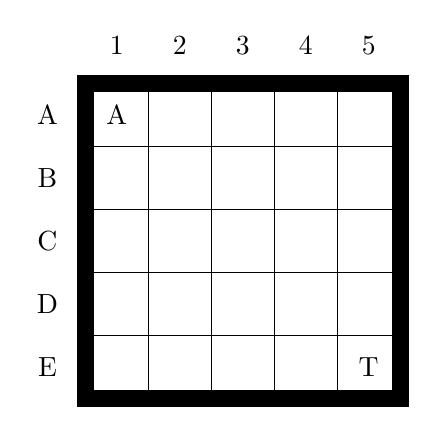
\begin{tikzpicture}[x=0.8cm,y=0.8cm]
  % --- outer thick border (5x5) ---
  \draw[line width=6pt] (0,0) rectangle (5,5);

  % --- inner grid lines ---
  \foreach \i in {1,2,3,4} {
    \draw (\i,0) -- (\i,5);
    \draw (0,\i) -- (5,\i);
  }

  % --- column labels 1..5 (top) ---
  \foreach \c in {1,2,3,4,5} {
    \node at (\c-0.5, 5.6) {\c};
  }

  % --- row labels A..E (left), top to bottom ---
  \foreach \r/\lab in {4.5/A,3.5/B,2.5/C,1.5/D,0.5/E} {
    \node at (-0.6, \r) {\lab};
  }

  % --- cell contents ---
  \node at (0.5,4.5) {A};  % top-left cell
  \node at (4.5,0.5) {T};  % bottom-right cell
\end{tikzpicture}

\textbf{Assg 1 - Figure 9 Maze}
\end{center}

\noindent
For the following analysis we will focus on the maze presented in Figure 9 from the Assignment 1 write-up.
\\

\noindent The figure 9 maze is a great maze to analyze due to it having no walls. When running both forms of cell expansion prioritization, the following results can be observed. 

\begin{center}
\begin{tabular}{|l|r|r|r|r|}
\hline
\textbf{Maze} & \textbf{Large G Cells Exp.} & \textbf{Small G Cells Exp.} & \textbf{Large G Time (s)} & \textbf{Small G Time (s)} \\
\hline
Figure 9 & 8 & 24 & 0.0002 & 0.0001 \\
\hline
\end{tabular}
\end{center}

\noindent \textbf{Background}: The heuristic value computed by Repeated Forward A* is based on the Manhattan distance between each cell $S$ and the end $T$. Due to no walls existing within this maze, all cells end up sharing the same f-value. This creates a f-value plateau, where tie breaking becomes the factor determines which $S$ the search will prioritize expanding.
\[ f = g + h\]

\noindent Repeated Forward A* computes the f-value of a cell using the above formula. $g$ is the value of the shortest possible path from the starting point $A$ to some possible state $S$. $h$ is the heuristic value, calculated by using Manhattan distance, that estimates the distance from state $S$ to the goal $T$. \\

\noindent \textbf{Smallest g-value}: When expansion ties are broken in favor of $S$ that have the smallest g-values (+1 being provided as the sign parameter), A* will expand states in increasing g-value order. This results in a BFS-style expansion, where the algorithm explores the gridworld layer by layer from the provided start state. The smallest g-values will always be closest to the starting point which results in the search expanding most, if not all, possible states.\\

\noindent \textbf{Largest g-value}: When ties are broken instead in favor of the highest g-values (-1), A* will implicitly prioritize all possible states $S$ that are closer to the goal $T$. In an f-value plateau such as that in the Figure 9 maze, a larger g-value will result in the h-value being much shorter. A smaller h-value means the corresponding state is closer to the goal $T$. Larger g-value priority results in the A* search being aggressive and exploring states that are inherently closer to $T$. This typically results in a reduction in cells expanding in contrast to the path taken by prioritizing states with smaller g-values.\\

\noindent \textbf{Conclusion}: The observations seen with Figure 9 are backed up by the results found in the 50 gridworlds analyzed earlier. If a maze has a lot of dead ends, such as the one in Maze 4, prioritizing by large g-values may result in dead ends being hit more often. This can be explained by the agent not having world knowledge and always assuming any unseen cells are empty. This does sometimes result in dead ends being hit, thus expanding the number of cells explored, however the overall performance of large g-value prioritization is significantly better than the small g-value counterpart. 
\\ \\

\noindent 
\section*{Question 5: Repeated Forward A* and Adaptive A* using Heuristics}

\subsection*{Methodology}
We implemented one version of the Repeated Forward A* algorithm with a variable that determined the cell prioritization: 

\begin{itemize}
    \item \textbf{Repeated Forward A*}: The same Repeated Forward A* implementation used in Q2 is used for this question, with the only difference being ties are always broken by the Largest g-values first, then randomly.
    \item \textbf{Adaptive A*}: Similar implementation to Repeated Forward A* with an important addition: the search now stores and updates the h-values of expanded states. These updated h-values are then used to make better expansion choices in future iterations of Repeated Forward A*. Overtime the h-values become more accurate, which reduces the number of states expanded, essentially adapting with each search, hence the name. 
\end{itemize}

\begin{center}
\begin{tabular}{|l|r|r|r|r|r|}
\hline
\textbf{Maze} & \textbf{Solvable} & \textbf{Fwd Cells Exp.} & \textbf{Adp Cells Exp.} & \textbf{Fwd Replans} & \textbf{Adp Replans}\\
\hline
Maze 0  & False & 22906  & 23497 & 142 & 152 \\
Maze 1  & False & 17763 & 17863 & 79  & 80  \\
Maze 2  & False & 17085 & 17057 & 83  & 84  \\
Maze 3  & True  & 13190 & 11701 & 135 & 132 \\
Maze 4  & True  & 9605   & 9815  & 96  & 101 \\
... & ... & ... & ... & ... & ... \\
Maze 49 & False & 1     & 1      & 0   & 0   \\
\hline
\textbf{Average} & \textbf{---} & \textbf{8637.8} & \textbf{8379.7} & \textbf{62.8} & \textbf{62.6} \\
\hline
\end{tabular}
\end{center}

\subsection*{Analysis}
\textbf{Observation:} Adaptive A* expanded about 3\% fewer cells than Repeated Forward A* on average. Adaptive cell implementation is used to reduce redundant cell explorations in multiple searches. The improvement isn't drastic because many of the generated mazes end up being unsolvable due to the agent immediately being blocked or requiring very few re-plans, thus limiting the opportunity for Adaptive A* to reuse information from prior searches. This issue ends up preventing adaptive search from displaying it's strongest benefit which is easily seen in mazes that require a lot of re-plans. \\

\begin{center}
\begin{tabular}{|l|r|r|r|r|r|}
\hline
\textbf{Maze} & \textbf{Solvable} & \textbf{Fwd Cells Exp.} & \textbf{Adp Cells Exp.} & \textbf{Fwd Replans} & \textbf{Adp Replans}\\
\hline
Maze 17  & False & 28001  & 23939 & 165 & 162 \\
Maze 19  & False & 13015 & 11638 & 125  & 108  \\
Maze 37  & True & 16214 & 14884 & 141  & 139  \\
...      & ...   & ...    & ...   & ... & ... \\
\hline
\end{tabular}
\end{center}

\noindent Adaptive A* improves performance by updating the heuristic values of previously expanded states. Constantly updating the h-values of expanded cells reflects the true cost-to-goal of a specific cell; further searches tend to become more focused on cells closer to the goal. Adaptive search is able to learn and guide future searches to be more goal-oriented than forward search. Forward search has the disadvantage of having to re-run A* search every time from scratch. \\

\noindent The observations made in the previous paragraph can be seen in the table above. Higher re-plan counts ultimately reduce the cell expansion count for adaptive search. Heuristic updates alter the exploration order and may even result in minor cell expansion count (such as in maze 0 or 1), but it typically reduces repeated work when re-planning.  \\

\noindent Adaptive A* search introduces the new issue of memory overhead. Adaptive search has to remember all h-values calculated for cells already expanded, which can become a memory-intensive job for extremely large mazes. Adaptive search must also be implemented properly to avoid bugs.



\end{document}